\section{Вычислительные эксперименты}
    Возьмём параметры для модели:
    \[
        \begin{split}
            & \xi_1 = 10, \xi_2 = 8, \xi_3 = 6, \\
            & \alpha_{12} = 6, \alpha_{13} = 2, \alpha_{23} = 0.5, \\
            & k_{12} = 4, k_{13} = 1, k_{23} = 0.5.
        \end{split}
    \]

    При этом точка равновесия \( x^{(4)} = ( -3.458\dots, 46.66\dots, -150 ) \). Откуда получаем \( b_3 = -22040 \Rightarrow \Delta_2 = 22040 > 0 \). Значит, что по какой-то оси она будет устойчивая, по второй неустойчива, а по третьей устойчивость неизвестна. Однако, вероятно, это точка не будет иметь влияния, поскольку находится на большом удалении в отрицательных координатах.

    \subsection{При вымершей первой популяции}

    \begin{figure}[H]
        
        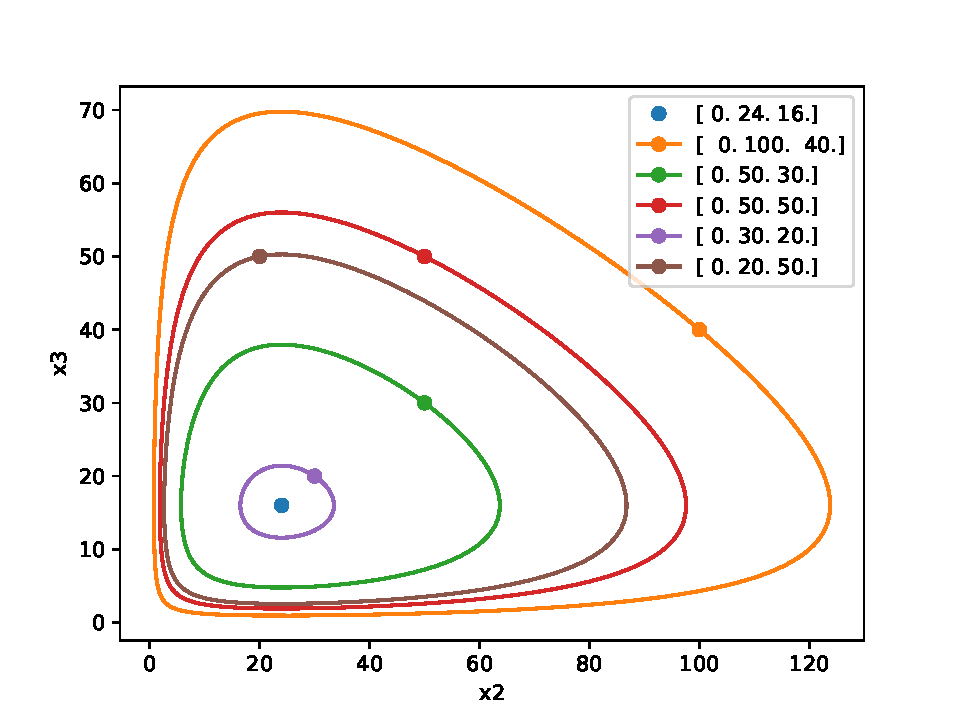
\includegraphics[width=8cm]{pictures/x1_0phase.pdf}
        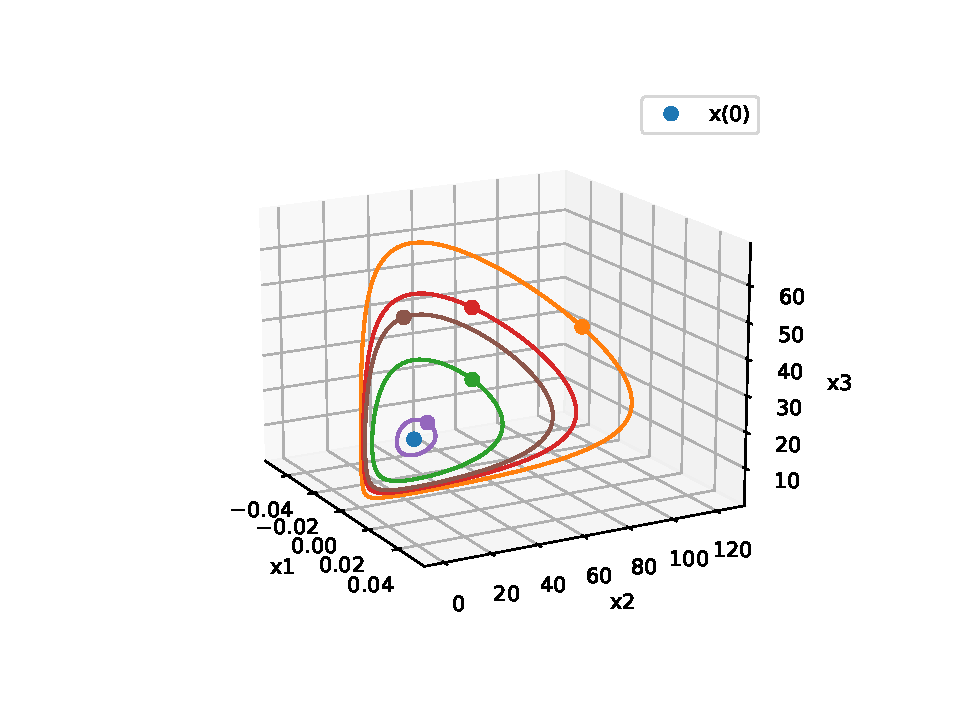
\includegraphics[width=8cm]{pictures/x1_0phase3.pdf}
        \caption{На отрезке времени \( [0, 3] \).}
    \end{figure}


    \subsection{При вымершей второй популяции}

    \begin{figure}[H]
        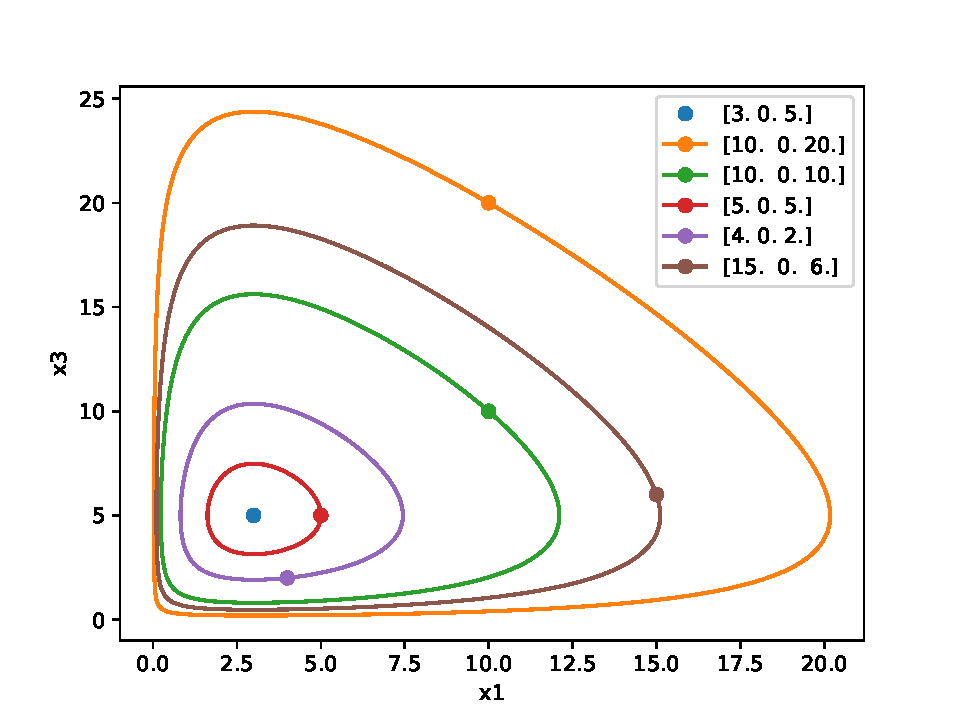
\includegraphics[width=8cm]{pictures/x2_0phase.pdf}
        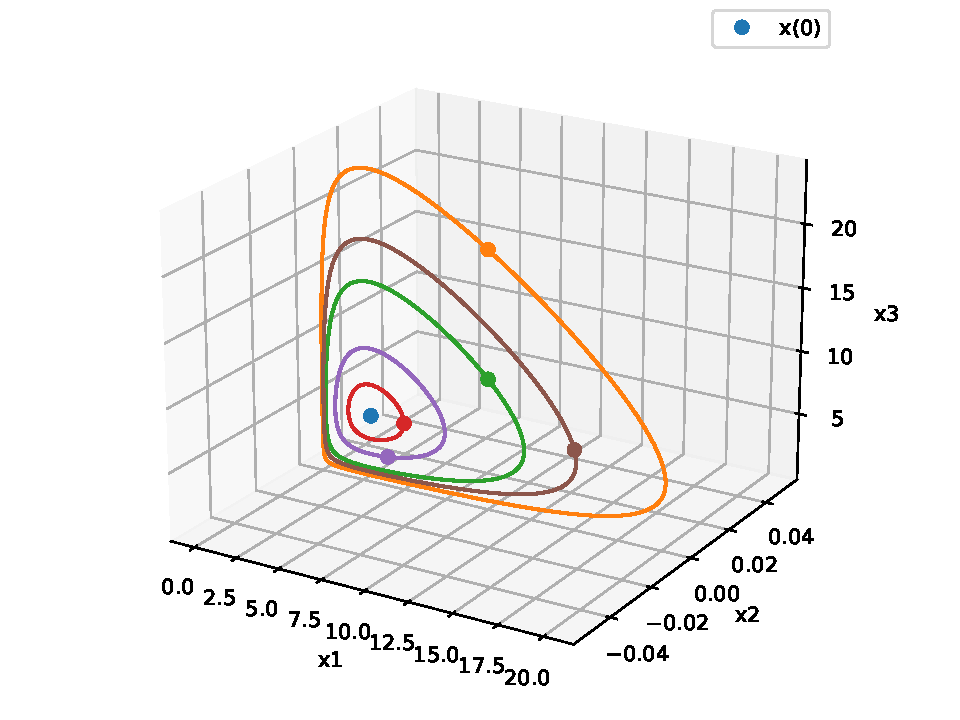
\includegraphics[width=8cm]{pictures/x2_0phase3.pdf}
        \caption{На отрезке времени \( [0, 3] \).}
    \end{figure}


    \subsection{При вымершей третьей популяции}

    \begin{figure}[H]
        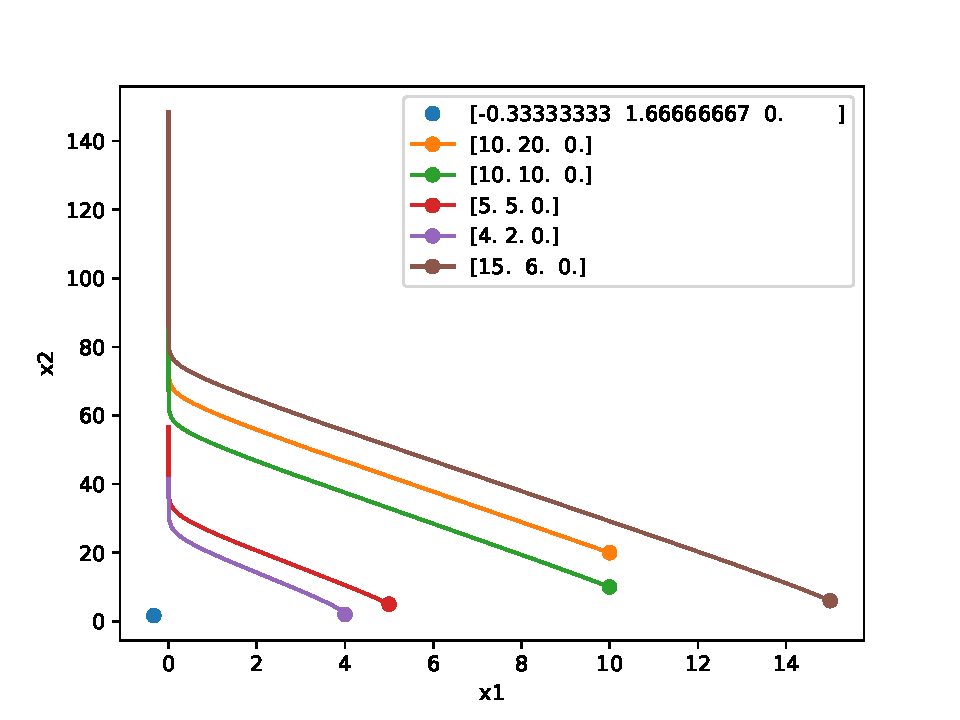
\includegraphics[width=8cm]{pictures/x3_0phase.pdf}
        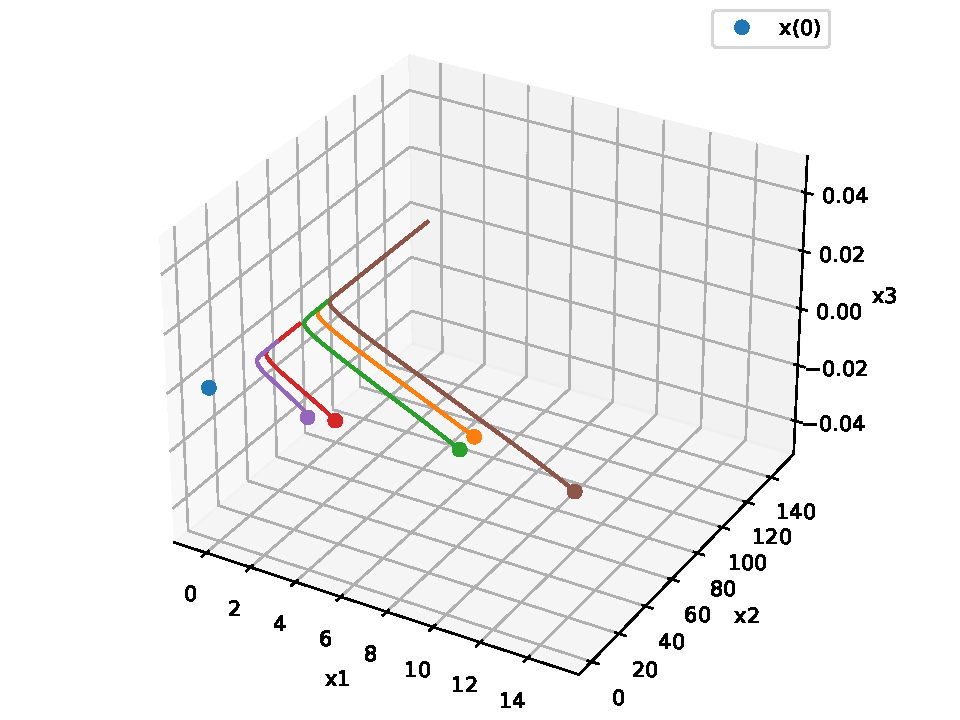
\includegraphics[width=8cm]{pictures/x3_0phase3.pdf}
        \caption{На отрезке времени \( [0, 0.1] \).}
    \end{figure}

    \subsection{Несколько изначально не вымерших популяций}
    \begin{figure}[H]
        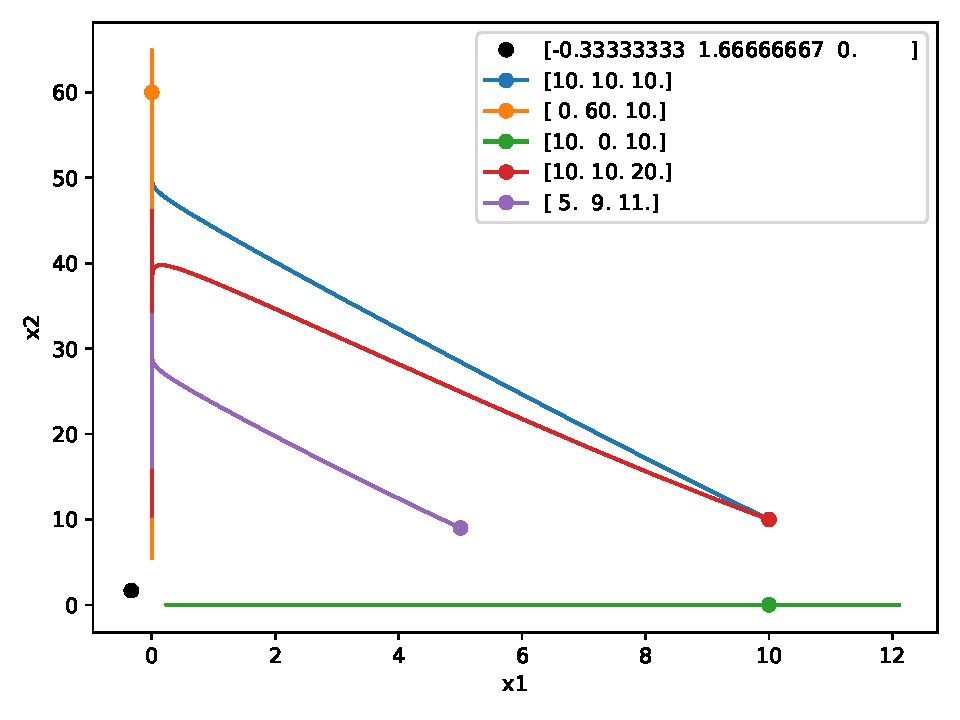
\includegraphics[width=8cm]{pictures/x_12phase.pdf}
        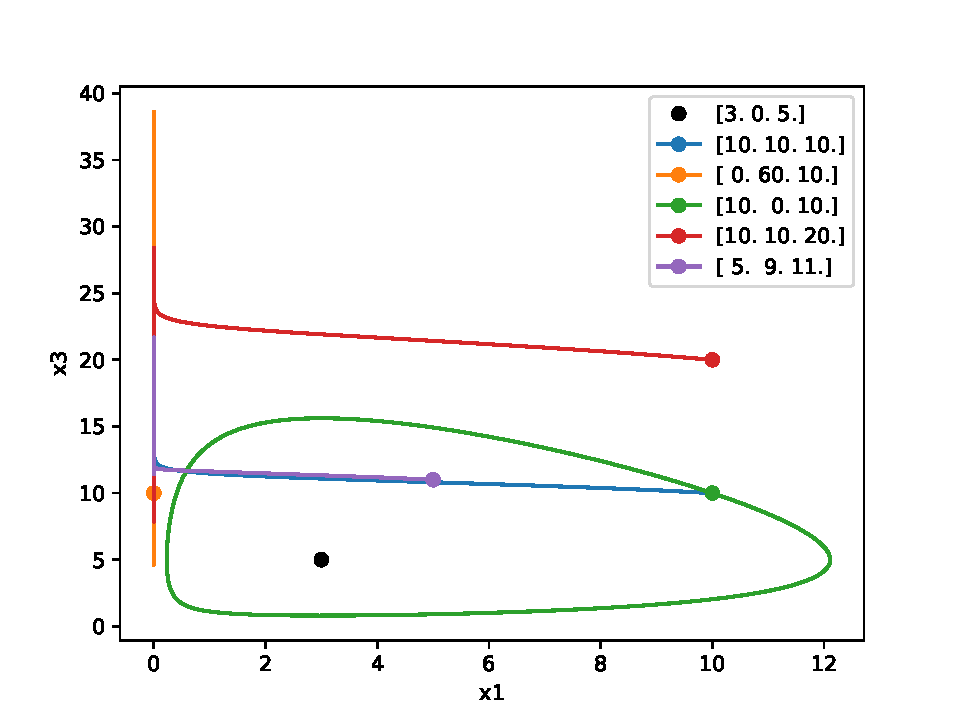
\includegraphics[width=8cm]{pictures/x_13phase.pdf}
        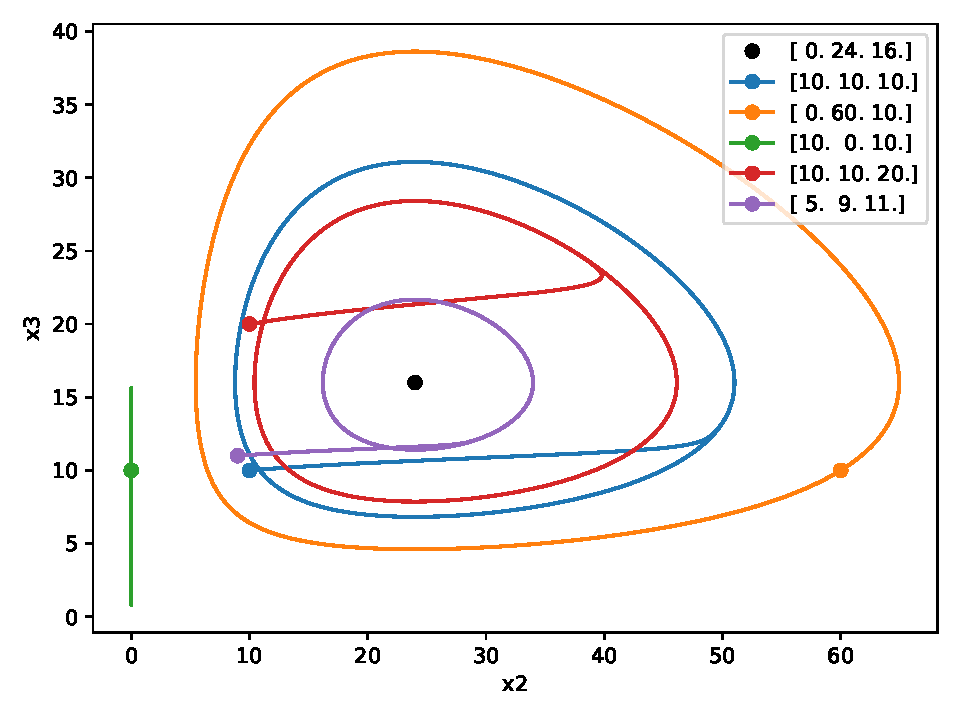
\includegraphics[width=8cm]{pictures/x_23phase.pdf}
        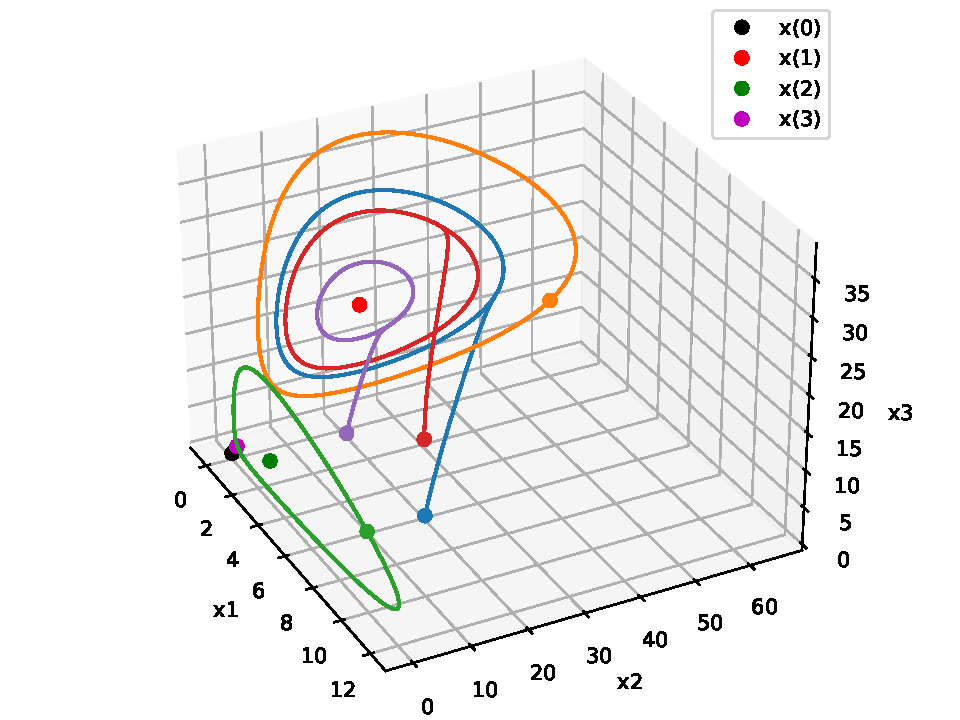
\includegraphics[width=8cm]{pictures/x_phase3.pdf}
        \caption{На отрезке времени \( [0, 3] \).}
    \end{figure}